% !TEX root = MAIN.tex

\section{MASS}

\subsection{Software static architecture}





\begin{figure}[h]
  \centering
	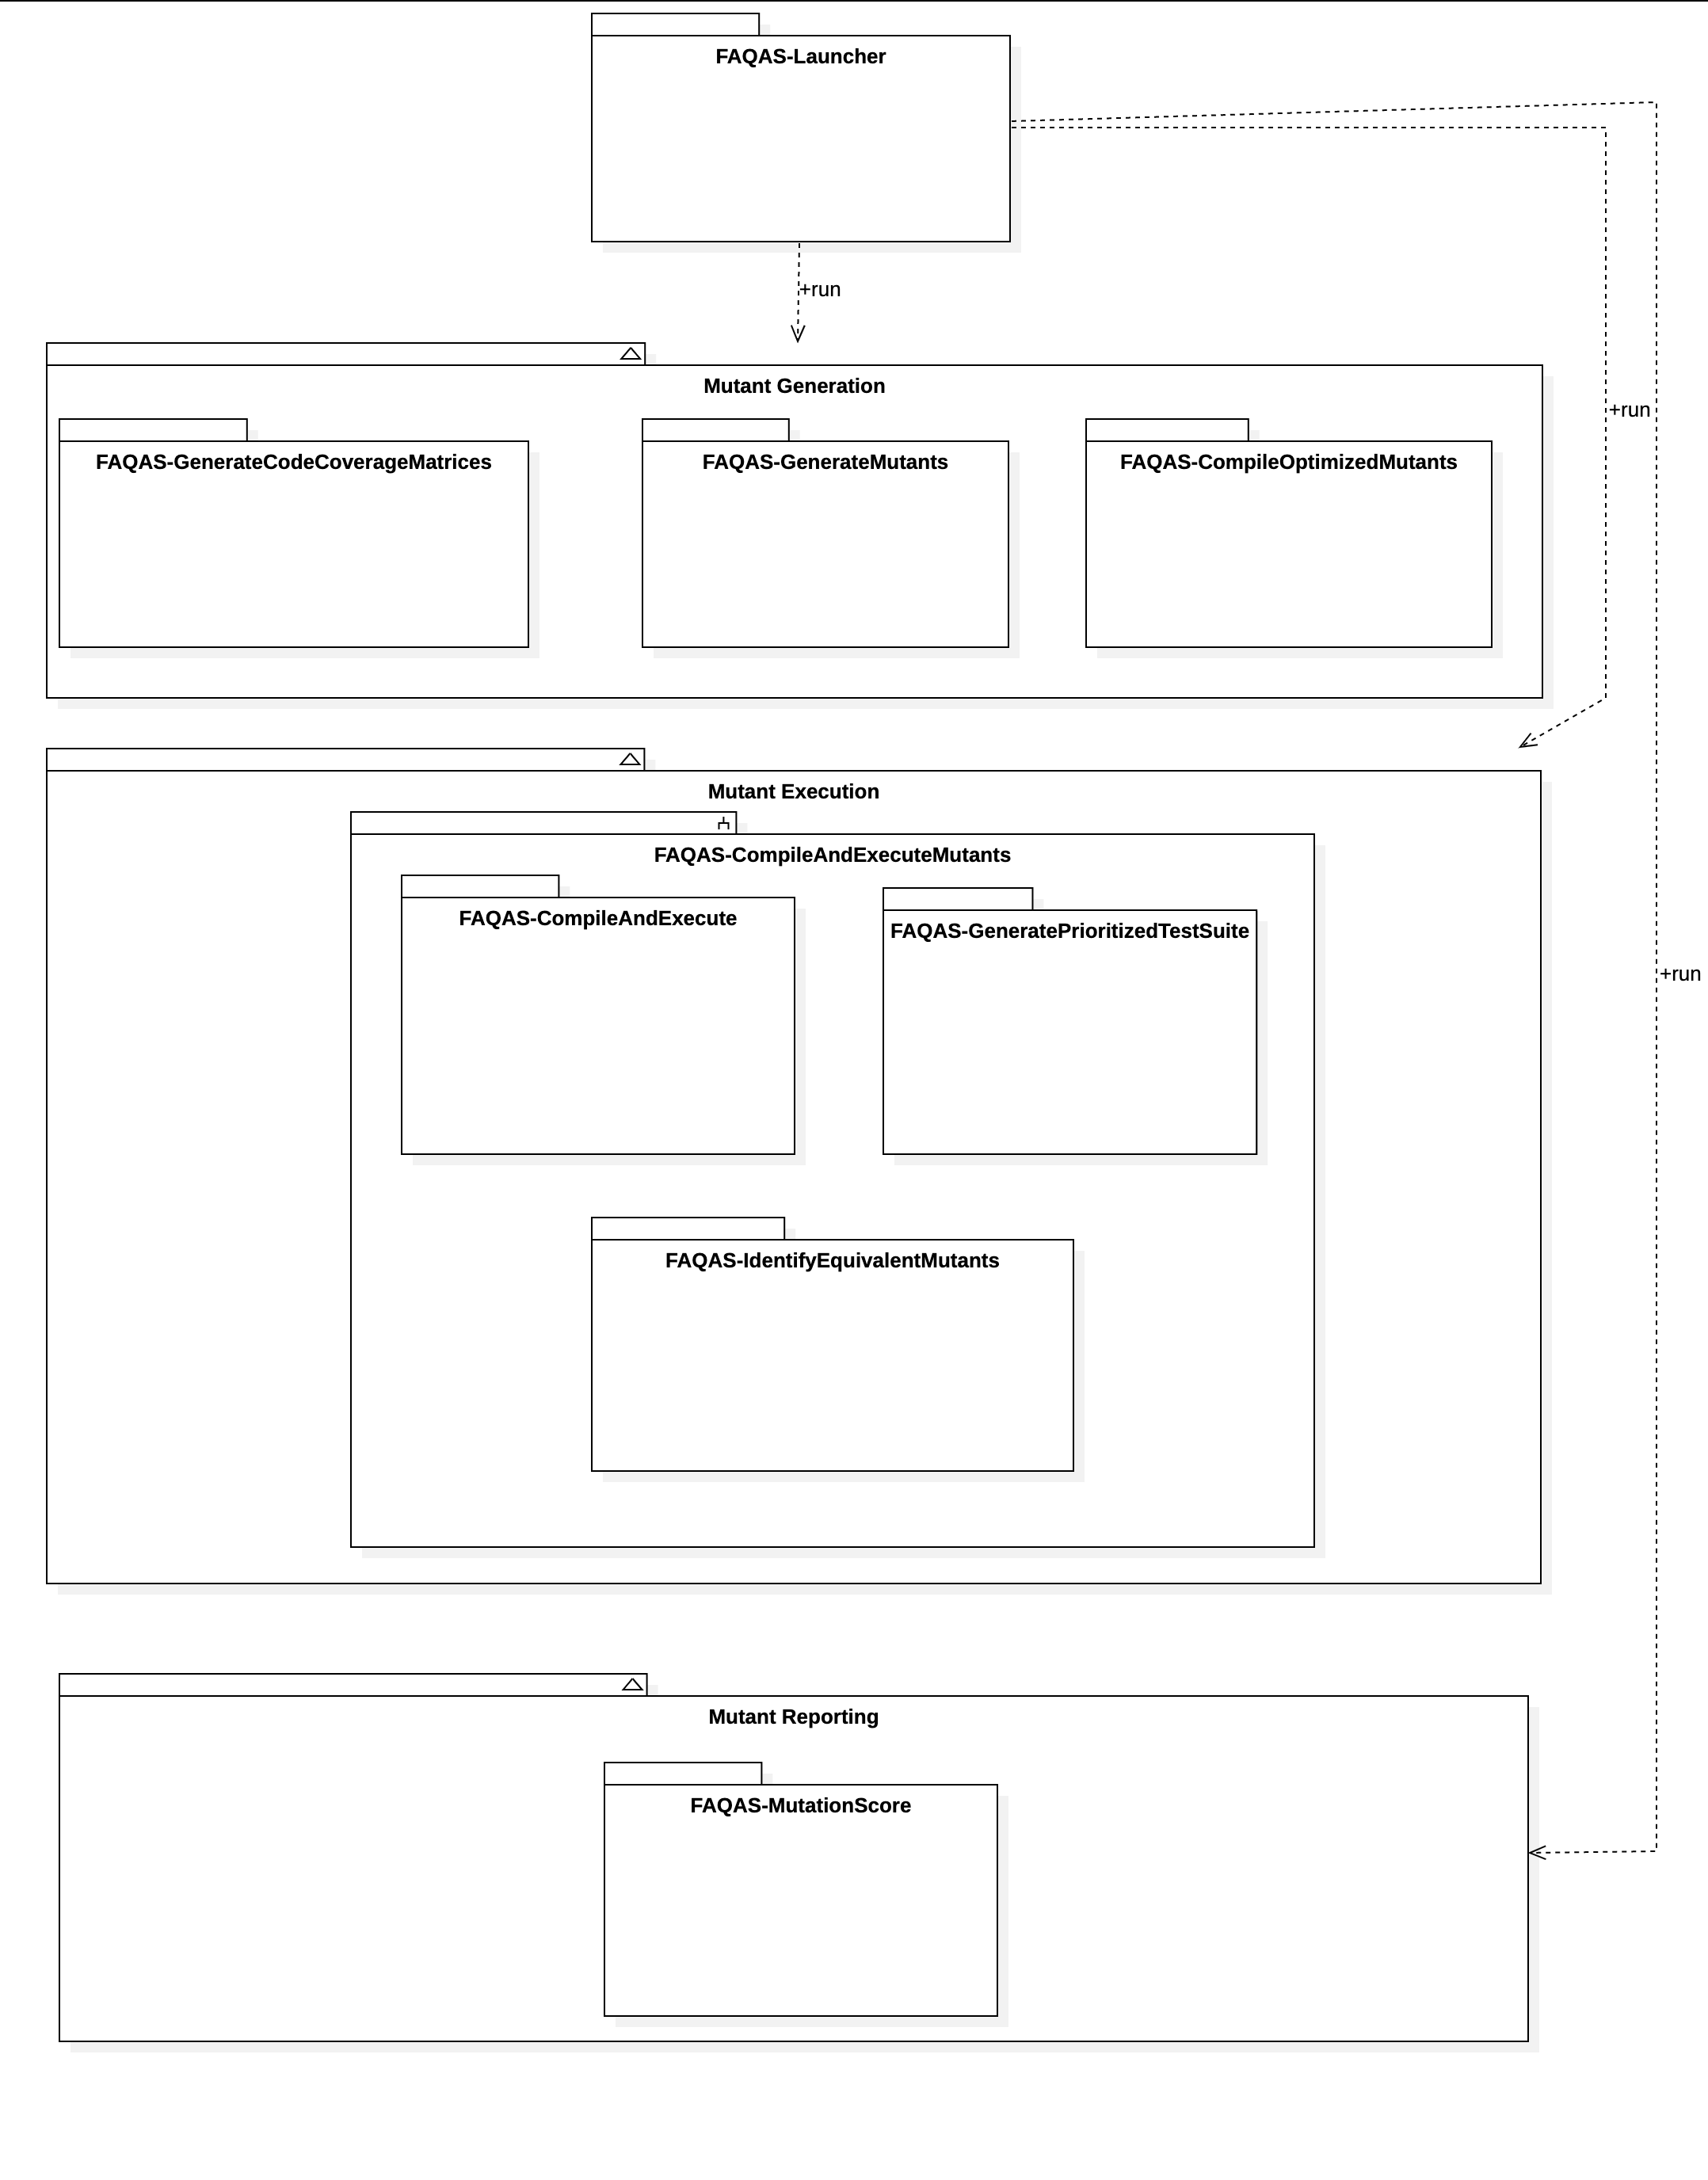
\includegraphics[width=0.8\textwidth]{images/static_architecture.png}
      \caption{UML Architecture diagram of MASS.}
      \label{fig:architecture_diagram}
\end{figure}

The architecture of the code-driven mutation analysis toolset (i.e., MASS)  is drafted in Figure~\ref{fig:architecture_diagram}.
Figure~\ref{fig:architecture_diagram} relies on UML package diagram notation.

As depicted in Figure~\ref{fig:architecture_diagram}, the architecture of the component is divided in three packages, which are named \textit{Mutant Generation}, \textit{Mutant Execution}, and \textit{Mutant Reporting}. Also, it includes the entry point \textit{FAQAS-Launcher}.

The package \textit{Mutant Generation} implements the features concerning (1) the collection of code coverage, (2) the generation of mutants, and (3) the discarding of equivalent and redundant mutants based on compiler optimisations.

The package \textit{Mutant Execution} implements the features regarding the compilation and execution of mutants. Note that this layer implements also the strategies for mutation sampling and reduction of the test suites.

The package \textit{Mutant Reporting} implements the features for the generation of the mutation analysis reports including the mutation score.


\subsubsection{Source Code Structure}


\REVISION{P-00}{ \MASS is delivered as a compressed archive consisting of source files and an installer.
The following bulletpoints provide a description of the archive's structure once uncompressed:

\begin{itemize}
	\item \texttt{MASS/}
	\begin{itemize}
		\item \texttt{SRCMutation/}: contains the source files and unit test cases of the component that performs code-driven mutations.
		\item \texttt{llvm-build.sh}: build script that compiles the SRCMutation component
		\item \texttt{PythonWrappers/}: contains Python script wrappers that facilitate code-driven mutations.
		\item \texttt{MASS/}: contains all the executable files and scripts that implement the methodology for code-driven mutation testing supported by the \MASS. They are listed below.
		\begin{itemize}
			\item \texttt{FAQAS-Setup}: contains the Bash scripts necessary to install the FAQAS-Framework.
			\item \texttt{FAQAS-GenerateCodeCoverageMatrixes}: contains the Bash scripts providing procedures to collect code coverage from the SUT.
			\item \texttt{FAQAS-GenerateMutants}: contains a Bash script that invokes the \texttt{SRCMutation} component to generate mutants.
			\item \texttt{FAQAS-CompileOptimizedMutants}: contains the scripts (in Python and Bash)  that provide the procedures to compile mutants and filter equivalent and redundant mutants based on trivial compiler optimizations.
			\item \texttt{FAQAS-CompileAndExecuteMutants}
			\begin{itemize}
				\item \texttt{FAQAS-GeneratePrioritizedTestSuite}: contains the Python and Bash scripts that provide the procedures to generate prioritized and reduced test suites from the SUT.

				\item \texttt{FAQAS-CompileAndExecute}: contains the Python and Bash scripts that provide the procedures to compile and execute the mutants against the SUT test suite. It also provides the procedures to determine the mutation stopping criterion (i.e., mutant sampling).

				\item \texttt{FAQAS-IdentifyEquivalentAndRedundantMutants}: contains the Python and Bash scripts that provides the procedures to identify equivalent mutants based on code coverage.
			\end{itemize}
			\item \texttt{FAQAS-MutationScore}: contains the Python and Bash scripts that provide the procedures to compute the mutation score and provide summarized information about the code-driven mutation testing process.
		\end{itemize}
	\end{itemize}
\end{itemize}
}
\clearpage

\subsection{Software components design}

\begin{figure}[tb]
  \centering
	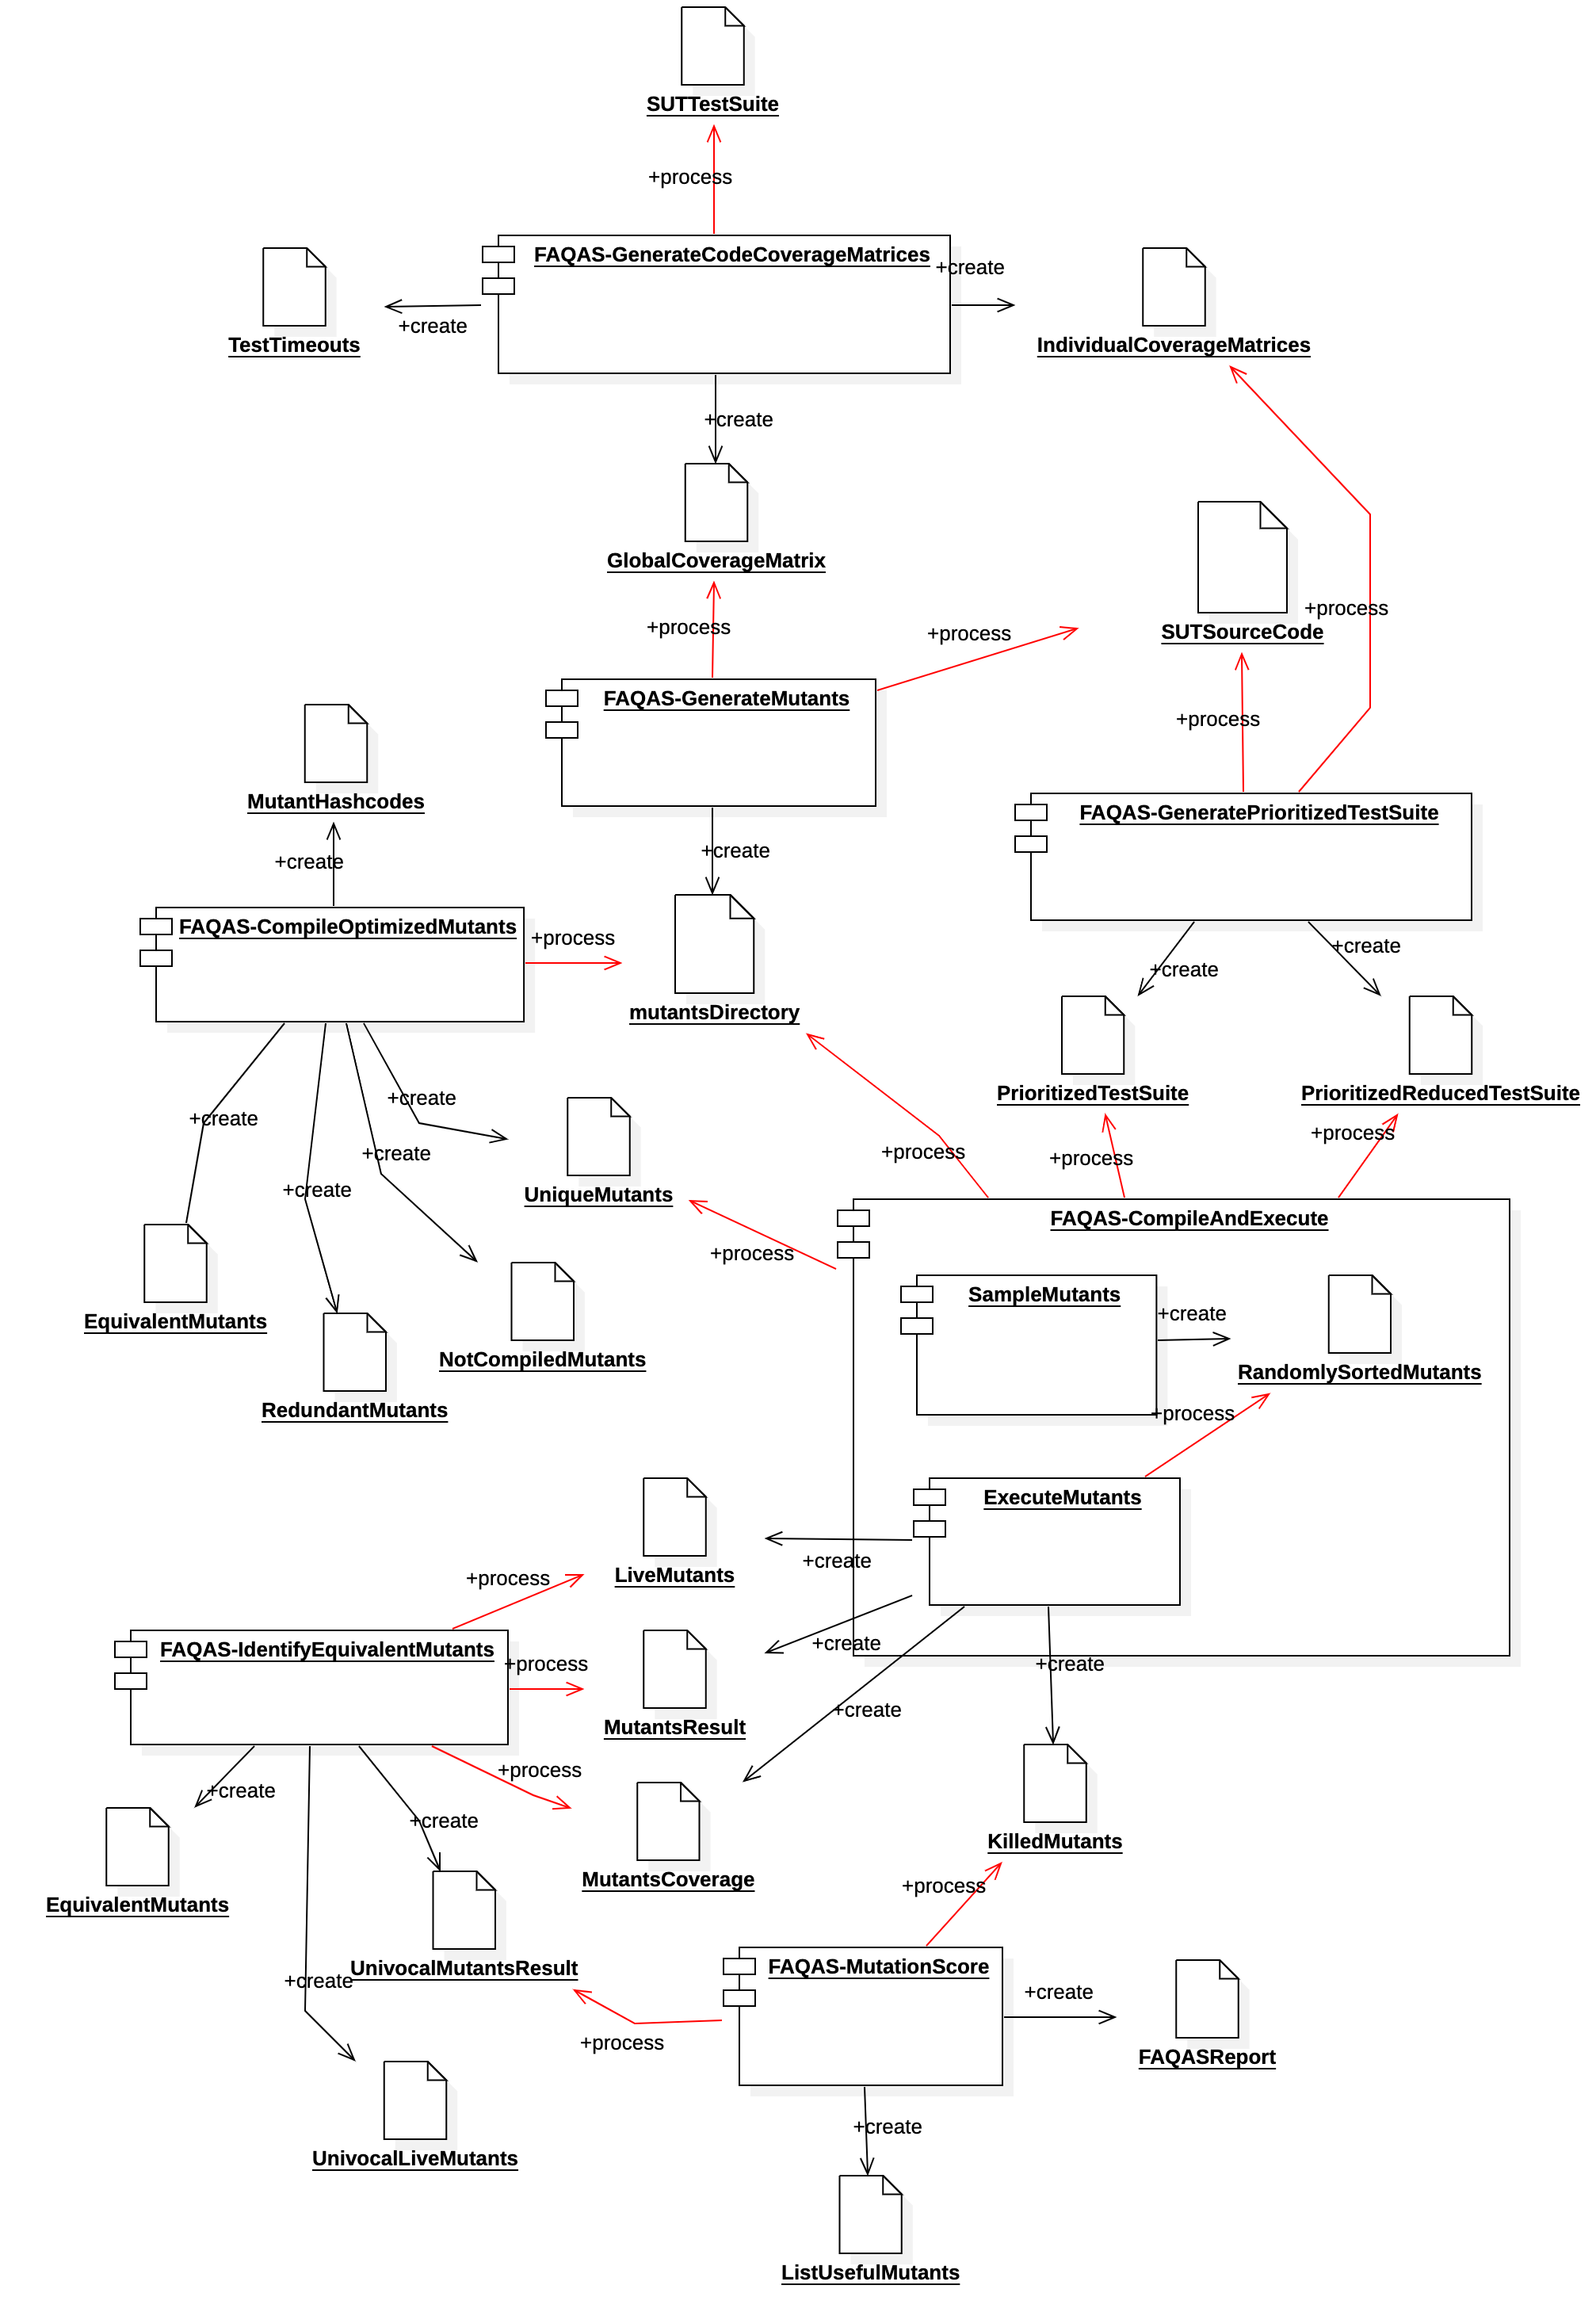
\includegraphics[width=0.9\textwidth]{images/component.png}
      \caption{UML Component diagram of the code-driven mutation testing component to evaluate test suite effectiveness.}
      \label{fig:component_diagram}
%      \DONE{Replace "creates" with "create".}
%            \DONE{Maybe yo can make "process" arrows red to make the data-flow more explicit?}
\end{figure}

The components of MASS are drafted in Figure~\ref{fig:component_diagram}. Figure~\ref{fig:component_diagram} relies on UML component diagram notation.

As shown in Figure~\ref{fig:component_diagram}, the software is composed by the following components:

\begin{itemize}
	\item \textit{FAQAS-GenerateCodeCoverageMatrices}: this component processes the SUT test suite and generates the files \textit{GlobalCoverageMatrix}, \textit{IndividualCoverageMatrices}, and \textit{TestTimeouts}. The information produced by the component is mainly processed by the \textit{FAQAS-GenerateMutants} component.
	
	\REVISION{P-1b}{
	\begin{itemize}
		\item \textit{GlobalCoverageMatrix}: csv file containing one line per source under test. The structure of each line is name of the source file, followed by a list with the coverage frequency for all the statements within that source file. Lines that cannot be covered are represented by a '-' character. For example, the coverage line:

		\texttt{source.c:-,-,-,1,4,4,-,0,1,0} 
		
		Indicates that the source \texttt{source.c} contains 10 lines, where the fourth line has been covered one time, and the fifth line has been covered four times.

		\item \textit{IndividualCoverageMatrices}: one csv coverage matrix file for each test case of the test suite. The structure of the file is identical to the \textit{GlobalCoverageMatrix}.
		\item \textit{TestTimeouts}: csv file containing one line per test case. The structure of each line is the name of the test case, followed by the test execution time times three, in seconds. For example, the line \texttt{acos:6} indicates that the test case \texttt{acos} cannot be executed for more than six seconds.
	\end{itemize}
	

	\item \textit{FAQAS-GenerateMutants}: This component processes the SUT source code and the \textit{GlobalCoverageMatrix} file, and generates the mutants directory.
		

	\item \textit{FAQAS-GeneratePrioritizedTestSuite}: this component processes the source code and the \textit{IndividualCoverageMatrices}, and produces two files: the \textit{PrioritizedTestSuite} and the \textit{PrioritizedReducedTestSuite}.

	\begin{itemize}
		\item \textit{PrioritizedTestSuite}: csv file containing one line per each covered line of the SUT. The structure of each line is the name of the source file, the line number, followed by a list of prioritized test cases to be executed. Each test case indicates the coverage distance estimated as the cosine distance of the coverage profile. For example, the line:

		\texttt{source.c|54|test5:0;test3:0.03;test2:0.01;test1:0.003;test4:0.0}

		Indicates that mutants affecting \texttt{source.c} on line 54 shall be executed first against \texttt{test5}, followed by \texttt{test3}, \texttt{test2}, \texttt{test1}, and finally \texttt{test4}.

		\textit{PrioritizedReducedTestSuite}: csv file containing one line per each covered line of the SUT. The structure of each line is the name of the source file, the line number, followed by a list of prioritized and reduced test cases to be executed. The structure is identical to the \textit{PrioritizedReducedTestSuite}.
	\end{itemize}

	\item \textit{FAQAS-CompileOptimizedMutants}: this component processes the mutants directory and produces five files:
	\begin{itemize}
		\item \textit{MutantHashcodes}: File containing the list of hash-codes for each mutant, the file contains one line per mutant. The structure of each line is the name of the mutant, the original source of the mutant, and the hash code of the compiled mutant. An example follows:

		\texttt{source.mut.126.1\_6\_19.ICR.function\_1;src/source.c;947899b54fe9eb785}

		\item \textit{UniqueMutants}: file containing the list of nonequivalent and nonredundant mutants, each line contains the name of the mutant followed by the original source of the mutant. An example follows:

		\texttt{source.mut.126.1\_6\_19.ICR.function\_1|src/source.c}
		
		\item \textit{EquivalentMutants}: File containing the list of equivalent mutants. The structure of the file is identical to \textit{UniqueMutants}.
		
		\item \textit{RedundantMutants}: File containing the list of redundant mutants. The structure of the file is identical to \textit{UniqueMutants}.
		
		\item \textit{NotCompiledMutants}: File containing the list of non-compiled mutants. The structure of the file is identical to \textit{UniqueMutants}.
	\end{itemize}
	\item \textit{FAQAS-CompileAndExecute}: this component is composed by two sub-components:
		\begin{itemize}
			\item \textit{SampleMutants}: this component processes the file \textit{UniqueMutants} and generates the file \textit{RandomlySortedMutants}.

			\begin{itemize}
				\item \textit{RandomlySortedMutants}: File containing one line per each sampled mutant. The structure of the file is identical to \textit{UniqueMutants}.
			\end{itemize}
			\item \textit{ExecuteMutants}: this component processes the file \textit{RandomlySortedMutants}, and execute the mutants (according to the strategy selected by the end-user). It produces the following files:
			\begin{itemize}
				\item \textit{LiveMutants}: file containing the list of live mutants, it contains one line per live mutant. The structure of the file is identical to \textit{UniqueMutants}.
				
				\item \textit{KilledMutants}: file containing the list of killed mutants, it contains one line per killed mutant. The structure of the file is identical to \textit{UniqueMutants}.
				
				\item \textit{MutantsResults}: file containing the mutation traces, it contains one line per each test case executed against a mutant. Each line contains the name of the mutant, followed by the path of the original source, the compilation output (i.e., COMPILED/STILLBORN), the name of the executed test case, the test case outcome (i.e., PASSED/FAILED), the mutation output (i.e., LIVE/KILLED), and the execution time measured in milliseconds. An example follows:

				\stt{source.mut.211.2\_4\_9.UOI.function;src/source.c;COMPILED;test1;FAILED;KILLED;5593}
				
				\item \textit{MutantsCoverage}: folder containing the coverage for every mutant and each test case. The coverage is stored in gcov files (i.e., gcda and gcno files).
			\end{itemize}
		\end{itemize}

	\item \textit{FAQAS-IdentifyEquivalentMutants}: this component processes the files \textit{LiveMutants}, \textit{MutantsResults}, and \textit{MutantsCoverage}, and generates the files \textit{EquivalentMutants}, \textit{UnivocalLiveMutants}, and \textit{UnivocalMutantsResults}, that is, it filters equivalent mutants from the mutation execution process.
	\begin{itemize}
		\item \textit{EquivalentMutants}: file containing the list of equivalent mutants, that is, mutants with a coverage profile identical to the original program. The structure of the file is identical to \textit{UniqueMutants}.
		\item \textit{UnivocalLiveMutants}: file containing the list of live mutants, it contains one line per live mutant. The structure of the file is identical to \textit{UniqueMutants}.
		\item \textit{UnivocalMutantsResults}: file containing the filtered mutation traces, it contains one line per each test case executed against a mutant. The structure of the file is identical to \textit{MutantsResults}.

	\end{itemize}

	\item \textit{FAQAS-MutationScore}: this component processes the \textit{UnivocalMutantsResults} and the \textit{KilledMutants} files and produces the files \textit{FAQASReport} and \textit{LiveUsefulMutants}.

	\begin{itemize}
		\item \textit{FAQASReport}: text file containing information about \MASS mutation process. The information concerns total number of mutants generated, mutants filtered by TCE, type of sampling, total number of mutants executed, killed mutants, live mutants, mutation score, statement coverage, path to the \textit{LiveUsefulMutants} files.
		
		\item \textit{LiveUsefulMutants}: set of two csv files that contains one line per live mutant. The lists are sorted by the degree of coverage difference with respect to the original program. The structure of the file is identical to \textit{UniqueMutants}.
	\end{itemize}
	}
\end{itemize}

\clearpage

%\section{Software dynamic architecture}

\subsection{Software behavior}

%Concerning the dynamic behavior of the software, we introduce in the following descriptions for each of the four components of the \FAQAS: the Code-Driven Test Suite Evaluation and Augmentation, and the Data-Driven Test Suite Evaluation and Augmentation.

%\subsection{Code-Driven Test Suite Evaluation}

\begin{figure}[h]
  \centering
	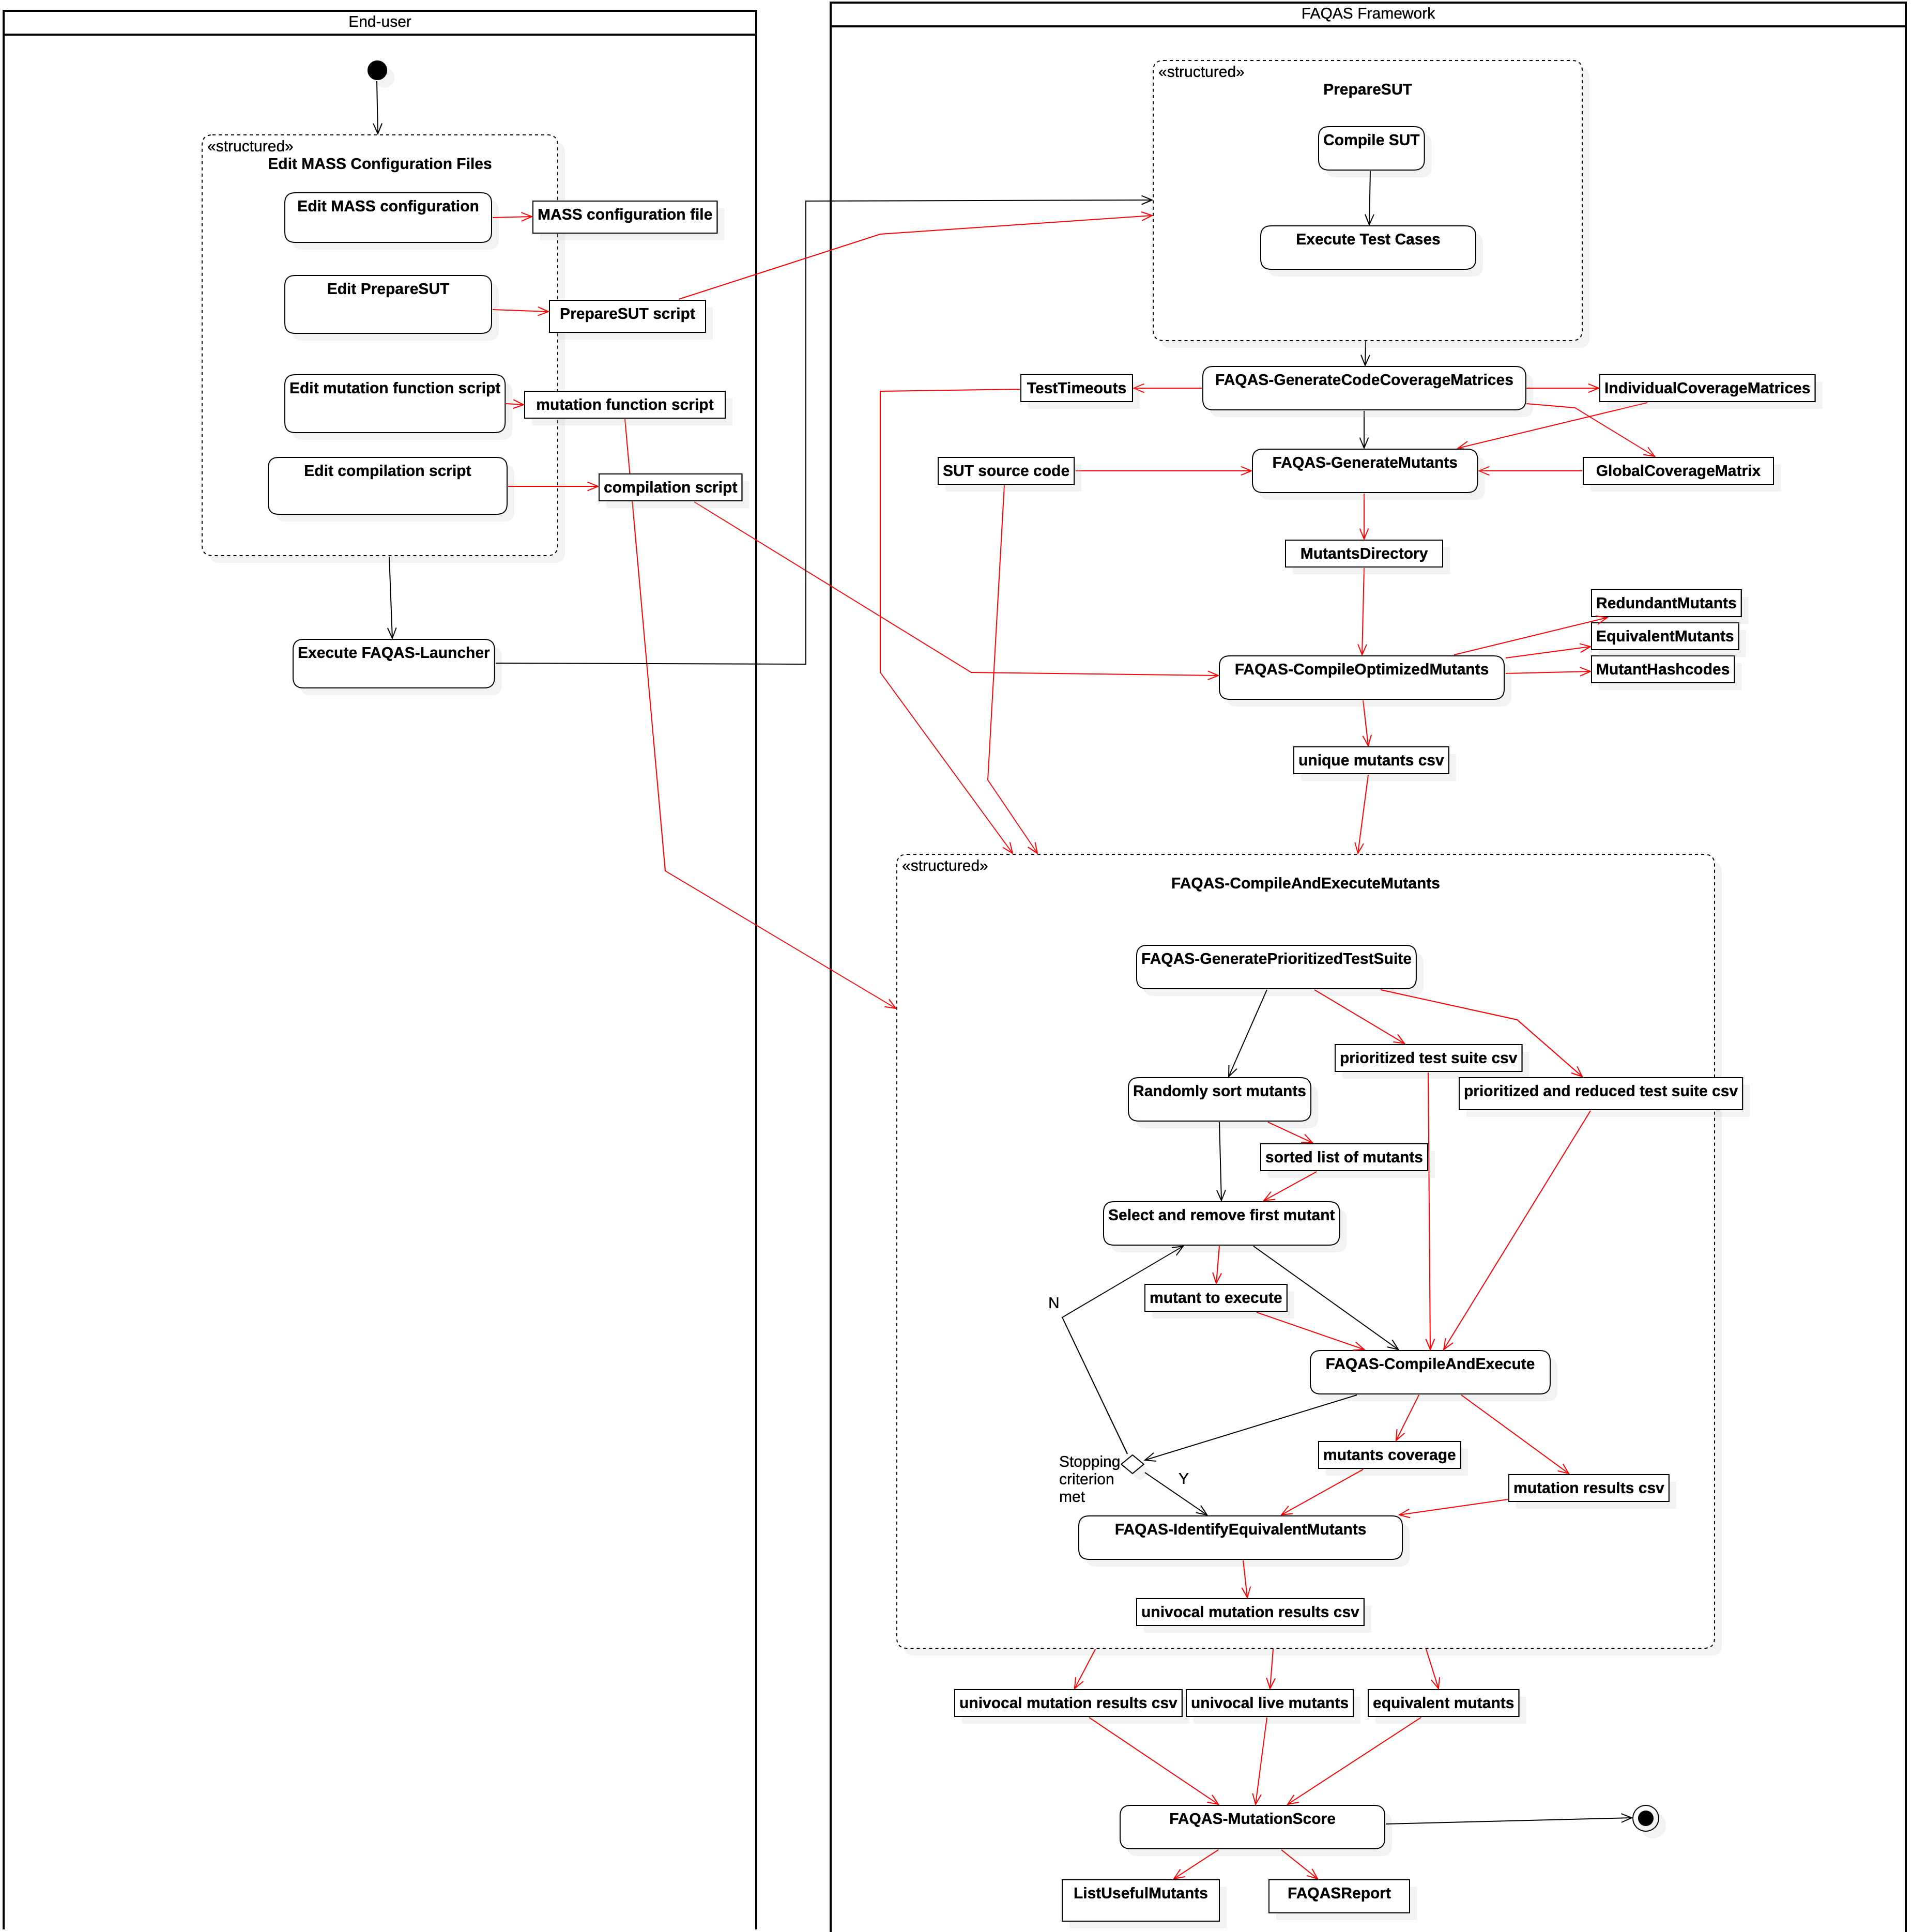
\includegraphics[width=\textwidth]{images/CodeDrivenTestSuiteEvaluation.png}
      \caption{Overview of the code-driven mutation testing process to evaluate test suite effectiveness.}
      \label{fig:process:codeDriven:evaluation}
\end{figure}


MASS implements the process for the evaluation of test suite effectiveness, drafted in Figure~\ref{fig:process:codeDriven:evaluation}. Figure~\ref{fig:process:codeDriven:evaluation} relies on UML activity diagram notation. In Figure~\ref{fig:process:codeDriven:evaluation} the execution of specific software artefacts from the end user is made explicit. Also, we use black arrows to draw control-flow, red arrows for data-flow. In the following, we further describe the evaluation of test suite effectiveness process.


The activity \emph{Edit MASS Configuration Files} indicates that the engineers must configure and perform the following activities:
\begin{itemize}
	\item Edit MASS configuration file: general configuration file
	\item Edit PrepareSUT script: script that compiles the SUT and executes the SUT test suite. In particular,  it extends the \emph{test suite script} for the SUT to store the code coverage of each single test case separately. This is achieved by adding a call to a dedicated bash script provided by FAQAS (\emph{FAQAS-CollectCodeCoverage}) after the execution of every test case.
	\item Edit Mutation function script: implementation of the function that executes the SUT test cases and decides whether a test case has been killed.
	\item Edit compilation script: modified version of the original build script to be used by \emph{FAQAS-}\emph{Compile\-OptimizedMutants}. The compilation script must be modified by:
	\begin{itemize}
	\item Removing debugging flags
	\item Removing coverage flags
	\item Adding a placeholder for the compiler optimization option
	\item Adding a 'sort' command in the source dependency list to ensure that source files are always compiled in the same order
	\end{itemize}
\end{itemize}

%\DONE{I think \emph{Prepare compilation scripts} is now covered by \emph{Edit compilation script} in the End-user part. I suggest to remove it from \emph{FAQAS-Framework part}. Also add the information above to the description of \emph{Edit compilation script}.}

The activity \emph{Compile SUT} in Figure~\ref{fig:process:codeDriven:evaluation} indicates that \MASS shall compile the SUT with coverage options enabled.

% The activity \emph{Prepare test scripts} in Figure~\ref{fig:process:codeDriven:evaluation} concerns extending the \emph{test suite script} for the SUT to store the code coverage of each single test case separately. This is achieved by adding a call to a dedicated bash script provided by FAQAS (\emph{FAQAS-CollectCodeCoverage}) after the execution of every test case.

%\DONE{The \emph{Prepare test scripts} is manual. Thus it should not be part of FAQAS-Framework. However, I think it has been replaced by "Edit compilation script" or "Edit PrepareSUT", no?}

The activity \emph{Execute test cases} in Figure~\ref{fig:process:codeDriven:evaluation} concerns the execution of the test cases following the practice for the SUT (e.g., running the command \texttt{make test}).

The activity \emph{Execute FAQAS-GenerateCodeCoverageMatrix} in Figure~\ref{fig:process:codeDriven:evaluation} concerns the execution of a program delivered with the FAQAS framework (i.e., FAQAS-GenerateCodeCoverageMatrix).

%\DONE{Some output arrows departing from FAQAS-GenerateCodeCoverageMatrix are missing}

The activity \emph{Execute FAQAS-GenerateCodeCoverageMatrix} in Figure~\ref{fig:process:codeDriven:evaluation} generates a set of files:
\begin{itemize}
\item one csv file referred to as \emph{global coverage matrix}, which indicates, for every line of code of the SUT, the ID of the test cases that cover the line of code;
\item a number of files  referred to as \emph{individual coverage matrices}, one for each test case of the SUT. Each file indicates, for every line of code of the SUT, the number of times it has been covered during a single execution of the test case;
\item one file (\emph{TestTimeouts}) specifying, for each test case, a timeout value after which we shall consider a test case as hanging. The timeout value is generated by the system by triplicating the time taken by a test case launched in activity \emph{Execute test cases}.
\end{itemize}

Activity \emph{Execute FAQAS-GenerateMutants} in Figure~\ref{fig:process:codeDriven:evaluation} concerns the execution of the program \emph{FAQAS-GenerateMutants}.

The program \emph{FAQAS-GenerateMutants} automatically generates a number of copies of each source file. Each copy contains one mutant.

\emph{FAQAS-GenerateMutants} mutates source files implemented with C/C++ programming languages.

%\DONE{What about C++? I think we promised it...}
%\OSCAR{We haven't tried yet... since all case studies are written in C.}

\emph{FAQAS-GenerateMutants} generates mutants by applying a set of mutation operators that can be selected by the end-users.

\emph{FAQAS-GenerateMutants} implements the set of operators listed in Table~\ref{table:operators}

% !TEX root =  ../Main.tex

\newcommand{\op}{\mathit{op}}
\newcommand{\ArithmeticSet}{ \texttt{+}, \texttt{-}, \texttt{*}, \texttt{/}, \texttt{\%} }
\newcommand{\LogicalSet}{ \texttt{&&}, \texttt{||} }
\newcommand{\RelationalSet}{ \texttt{>}, \texttt{>=}, \texttt{<}, \texttt{<=}, \texttt{==}, \texttt{!=} }
\newcommand{\BitWiseSet}{ \texttt{\&}, \texttt{|}, \land }
\newcommand{\ShiftSet}{ \texttt{>>}, \texttt{<<} }


\begin{table}[h]
\caption{Implemented set of mutation operators.}
\label{table:operators} 
\centering
\scriptsize
\begin{tabular}{|@{}p{4mm}@{}|@{}p{2cm}@{\hspace{1pt}}|@{}p{11.1cm}@{}|}
\hline
&\textbf{Operator} & \textbf{Description$^{*}$} \\
\hline
\multirow{7}{*}{\rotatebox{90}{\emph{Sufficient Set}}}&ABS               & $\{(v, -v)\}$	\\
\cline{2-3}
&AOR               & $\{(\op_1, op_2) \,|\, \op_1, \op_2 \in \{ \ArithmeticSet \} \land \op_1 \neq \op_2 \} $       \\
&    			  & $\{(\op_1, \op_2) \,|\, \op_1, \op_2 \in \{\texttt{+=}, \texttt{-=}, \texttt{*=}, \texttt{/=}, \texttt{\%} \texttt{=}\} \land \op_1 \neq \op_2 \} $       \\
\cline{2-3}
&ICR               & $\{i, x) \,|\, x \in \{1, -1, 0, i + 1, i - 1, -i\}\}$           \\
\cline{2-3}
&LCR               & $\{(\op_1, \op_2) \,|\, \op_1, \op_2 \in \{ \texttt{\&\&}, || \} \land \op_1 \neq \op_2 \}$            \\
&				  & $\{(\op_1, \op_2) \,|\, \op_1, \op_2 \in \{ \texttt{\&=}, \texttt{|=}, \texttt{\&=}\} \land \op_1 \neq \op_2 \}$            \\
&				  & $\{(\op_1, \op_2) \,|\, \op_1, \op_2 \in \{ \texttt{\&}, \texttt{|}, \texttt{\&\&}\} \land \op_1 \neq \op_2 \}$            \\
\cline{2-3}
&ROR               & $\{(\op_1, \op_2) \,|\, \op_1, \op_2 \in \{ \RelationalSet \}\}$            \\
&				  & $\{ (e, !(e)) \,|\, e \in \{\texttt{if(e)}, \texttt{while(e)}\} \}$ \\
\cline{2-3}
&SDL               & $\{(s, \texttt{remove}(s))\}$            \\
\cline{2-3}
&UOI               & $\{ (v, \texttt{--}v), (v, v\texttt{--}), (v, \texttt{++}v), (v, v\texttt{++}) \}$            \\   
\hline
\hline
\multirow{5}{*}{\rotatebox{90}{\emph{OODL}}}&AOD               & $\{((t_1\,op\,t_2), t_1), ((t_1\,op\,t_2), t_2) \,|\, op \in \{ \ArithmeticSet \} $       \\ 
\cline{2-3}
&LOD               & $\{((t_1\,op\,t_2), t_1), ((t_1\,op\,t_2), t_2) \,|\, op \in \{  \} \}$       \\ 
\cline{2-3}
&ROD               & $\{((t_1\,op\,t_2), t_1), ((t_1\,op\,t_2), t_2) \,|\, op \in \{ \RelationalSet \} \}$       \\ 
\cline{2-3}
&BOD               & $\{((t_1\,op\,t_2), t_1), ((t_1\,op\,t_2), t_2) \,|\, op \in \{ \BitWiseSet \} \}$       \\ 
\cline{2-3}
&SOD               & $\{((t_1\,op\,t_2), t_1), ((t_1\,op\,t_2), t_2) \,|\, op \in \{ \ShiftSet \} \}$       \\ 
%\hline
%COR               & $\{(\op_1, \op_2) \,|\, \op_1, \op_2 \in \{ \texttt{\&\&}, \texttt{||}, \land \} \land \op_1 \neq \op_2 \}$            \\
\hline
\hline
\multirow{3}{*}{\rotatebox{90}{\emph{Other}}}&LVR			& $\{(l_1, l_2) \,|\, (l_1, l_2) \in \{(0,-1), (l_1,-l_1), (l_1, 0), (\mathit{true}, \mathit{false}), (\mathit{false}, \mathit{true})\}\}$\\
&&\\
&&\\
\hline
\end{tabular}

$^{*}$Each pair in parenthesis shows how a program element is modified by the mutation operator. Th eleft element of the pair is replaced with the right element. We follow standard syntax~\cite{kintis2018effective}. Program elements are literals ($l$), integer literals ($i$), boolean expressions ($e$), operators ($\op$), statements ($s$), variables ($v$), and terms ( $t_i$, which might be either variables or literals).
\end{table}

\emph{FAQAS-GenerateMutants} generates as output a directory tree (\emph{MutantsDirectory} in Figure~\ref{fig:process:codeDriven:evaluation}) that follows the structure of the source directory tree of the SUT. However, every source file is replaced by a folder; the folder has the same name of the file. The folder contains all the mutants generated for that file. Every mutant has a name that univocally identifies it. The mutant name results from the conjunction of the following information:
source file name, mutated function name, mutated line, mutation operator name, mutation operation, mutated ``column'' (i.e., char position from the beginning of the line).
In the following, we report the structure of the output directory generated for a program

\begin{verbatim}
./src/store/vmem/vmem_checksum_first.c
./src/log/telemetry_appender.c

./src-mutants/store/vmem/vmem_checksum_first/
vmem_checksum_first.mut.145.7_1_13.ROR.vmem_param_load.c
./src-mutants/log/telemetry_appender/
telemetry_appender.mut.116.3_1_18.ROR.gs_log_appender_telem_append_isr.c
\end{verbatim}

%\DONE{The "compilation script" should be an output of \emph{Edit compilation script}}

Activity \emph{Execute FAQAS-CompileOptimizedMutants} in Figure~\ref{fig:process:codeDriven:evaluation} concerns the execution of the program \emph{FAQAS-CompileOptimizedMutants}.

The program \emph{FAQAS-CompileOptimizedMutants} compiles every mutant multiple times, once for every compiler optimization option selected by the end-user. It implements the pseudocode in Figure~\ref{alg:CompileOptimizedMutants}.

\begin{figure}[h]
\begin{algorithmic}[1]

%\footnotesize
\scriptsize

\Require \emph{OPT}, the set of compiler optimization options specified by the end-user
\Require \emph{MutantsDir}, path of the directory tree containing the mutants
\Require \emph{SUTsources}, path of the folder containing the sources of the SUT
\Require \emph{CompilatonCommand}, the command to execute to compile the original software

\Ensure \emph{hashcodes csv}, a csv file containing for every mutant, for every option, the SHA512 hashcode of the generated executable

\Ensure \emph{unique mutants}, a csv file containing the list of unique mutants. Unique mutants are mutants that are not equivalent and not redundant. See D2 for details.

\For {OPT in OPTS}
\For {Mutant in MutantsDir}
\State Compile \emph{Mutant} with program \emph{FAQAS-CompileAndExecute}
\State Generate a SHA512 hash of the generated executable
\State Put the generated SHA512 hash in the \emph{hashcodes csv} file
\EndFor
\EndFor

\State Process \emph{hashcodes csv} and identify the \emph{unique mutants}
\State Save the list of \emph{unique mutants} in the output file \emph{unique mutants csv}

\end{algorithmic}
\caption{FAQAS-CompileOptimizedMutants: Algorithm for compiling mutants with multiple optimization options}
\label{alg:CompileOptimizedMutants}
\end{figure}


Activity \emph{Execute FAQAS-Compile\-And\-Execute\-Mutants} in Figure~\ref{fig:process:codeDriven:evaluation} concerns the execution of the program \emph{FAQAS-Compile\-And\-Execute\-Mutants}.

The program \emph{FAQAS-CompileAndExecuteMutants} iterates over three activities: \emph{FAQAS-Generate\-Prioritized\-Test\-Suite}, \emph{FAQAS-CompileAndExecute}, \emph{FAQAS-IdentifyEquivalentMutants}. Each activity is implemented by a dedicated executable program that is invoked automatically by \emph{FAQAS-CompileAndExecuteMutants} without user intervention.

The program \emph{FAQAS-CompileAndExecuteMutants} takes as inputs the \emph{mutants selection configuration}, the \emph{unique mutants csv}, the path of the \emph{SUT source folder}, the \emph{command to execute test cases}, and the \emph{path to the folder containing the test coverage matrices}.

The program \emph{FAQAS-CompileAndExecuteMutants} implements the four mutants selection strategies described in D2: \emph{all mutants}, \emph{proportional uniform sampling}, \emph{proportional method-based sampling}, \emph{uniform fixed-size sampling}, and \emph{uniform FSCI sampling}.

The \emph{mutants sampling configuration} consists of the mutants selection strategy and a configuration value that specifies the number of mutants to consider. The format of the value that specifies the number of mutants to consider depends on the strategy; the value may indicate the percentage of mutants to sample (for \emph{proportional uniform sampling}, \emph{proportional method-based sampling}), the number of mutants to sample (for \emph{uniform fixed-size sampling}).

The program\emph{FAQAS-GeneratePrioritizedTestSuite} takes as input the test coverage matrices and generates a file that specifies, for every line of the SUT, the prioritized list of test cases to execute (\emph{prioritized test suite csv}). This file indicates the sequence of test cases that shall be executed when testing a mutant affecting a certain line.

The activity \emph{Randomly sort mutants} indicates that  \emph{FAQAS-CompileAndExecuteMutants} generates a randomly sorted list of mutants. The list contains the mutants in \emph{unique mutants csv}.
In the case of \emph{proportional method-based sampling}, the list contains a set of mutants selected by following the stratified sampling strategy.

The activity \emph{Select and remove first mutant} indicates that  \emph{FAQAS-CompileAndExecuteMutants} selects the first mutant in \emph{sorted list of mutants} and removes it from the list.

The program \emph{FAQAS-CompileAndExecute} compiles a mutant by running the build script of the original program; then it executes the SUT test suite. It follows the algorithm in Figure~\ref{alg:compileAndExecute}.


\begin{figure}[h]
\begin{algorithmic}[1]
\scriptsize
\Require \emph{Mutant}, path of the mutant to compile
\Require \emph{SUTsources}, path of the folder containing the sources of the SUT
\Require \emph{CompilatonCommand}, the command to execute to compile the original software
\Require \emph{TestCommand}, the command to execute to execute a single test case
\Require \emph{TestCases}, the prioritized list of test cases for the line of the mutant
\Require \emph{TestTimeout}, the max execution time that can be taken by the test case
\Ensure \emph{Result} KILLED or LIVE, based on test execution result (i.e., all test cases pass or one test case fails)
\State put \emph{Mutant} in place of the file it has been derived (\emph{original file}), keep the original file in a safe place
\State execute  \emph{CompilatonCommand} inside \emph{SUTsources}
\For {TestCase in TestCases}
\State execute the \emph{TestCase} by running \emph{TestCommand} inside \emph{SUTsources}
% succede qualcosa strano quando scrivi "the"
\If {the \emph{TestCase} fails (i.e., \emph{TestCommand} terminates with an error code)}
\State set \emph{Result} as KILLED
\State break the for loop
\EndIf
\If {the \emph{TestTimeout} expires}
\State set \emph{Result} as KILLED
\State break the for loop
\EndIf
\EndFor
\State move code coverage information in a subfolder of \emph{mutants coverage dir}
\State restore the \emph{original file}
\end{algorithmic}
\caption{FAQAS-CompileAndExecute: Algorithm to compile and test mutants}
\label{alg:compileAndExecute}
\end{figure}

The program \emph{FAQAS-CompileAndExecute} collects the mutation results of every mutant in a file, i.e., \emph{mutation results csv}. It contains, for every mutant, the indication of the mutation result (KILLED/LIVE).

The program \emph{FAQAS-CompileAndExecute} compiles and executes mutants until a termination criterion is met. The termination criterion depends on the mutants selection strategy (see D2 for details):
\begin{itemize}
\item \emph{all mutants}: the list \emph{sorted list of mutants} is empty
\item \emph{proportional uniform sampling}: a number of mutants matching the selected percentage has been executed
\item \emph{proportional method-based sampling}: the list \emph{sorted list of mutants} is empty
\item \emph{uniform fixed-size sampling}: a number of mutants matching the selected value has been executed
\item \emph{uniform FSCI sampling}: the confidence interval computed from \emph{mutation results csv} is smaller than the length specified by the user.
\end{itemize}

The program \emph{FAQAS-IdentifyEquivalentMutants} relies on code coverage information stored in \emph{mutants coverage dir} to identify equivalent and redundant mutants using the distance criterion $D_C$ (see D2).

The program \emph{FAQAS-IdentifyEquivalentMutants} generates a copy of \emph{mutation results csv} (i.e., \emph{univocal mutation results csv}) where only mutants that are considered non-equivalent are reported.

The program \emph{FAQAS-MutationScore} concerns the computation of the mutation score based on the mutation results reported in \emph{univocal mutation results csv}, and the production of the two prioritized lists (list A and list B) of live and nonequivalent mutants (see FAQAS-SSS-REQ-051).


\subsection{Internal interface design}
\REVISION{P-1a}{
The internal interface design is limited to the interactions between different activities.

In general, each activity with a name starting with \emph{FAQAS-} is a wrapper. These wrappers do nothing by themselves other than calling an internal script.  

\subsection{External interface design}

The external interface design is limited to the interaction with a set of launchers that are provided in \MASS.

The set of launcher is composed by the following script files:

\begin{itemize}
	\item \texttt{PrepareSUT.sh}: launcher for the script that prepares the SUT and collects information about the SUT test suite.
	\item \texttt{GenerateMutants.sh}: launcher for the generation of mutants.
	\item \texttt{CompileOptimizedMutants.sh}: launcher for the trivial compiler optimization step.
	\item \texttt{OptimizedPostProcessing.sh}: launcher for the post-processing of the trivial compiler optimization step.
	\item \texttt{GeneratePTS.sh}: launcher for the generation of prioritized and reduced test suites.
	\item \texttt{ExecuteMutants.sh}: launcher for the execution of mutants against the SUT test suite.
	\item \texttt{IdentifyEquivalents.sh}: launcher for the identification of equivalent mutants based on code coverage.
	\item \texttt{MutationScore.sh}: launcher for the computation of the mutation score and final reporting.
	\item \texttt{PrepareMutants\_HPC.sh}: HPC launcher that prepares the mutants workspace for the execution on HPCs.
	\item \texttt{ExecuteMutants\_HPC.sh}: HPC launcher that executes mutants on HPCs.
	\item \texttt{PostMutation\_HPC.sh}: HPC launcher that assesses past mutant executions, and decides whether more mutant executions are needed.
\end{itemize}

\subsection{Test harness}

\MASS provide unit test cases for the \texttt{SRCMutation} component that generate mutants from the SUT source code. More information can be found in the \textit{ESA-FAQAS-SUITP} document.
}




